% !TEX root = C:\Users\Jan\Documents\dev\Risk-Measurement-Framework\masterthesis_tex\masterthesis_main.tex

\section{Risk-Measurement-Framework concept and design}
\label{sec:conFrame}

In contrast to Schwerdtner et al., the framework of this thesis concentrates on training, especially risk measurement before and during training of the ML model. The conceptual framework discusses and explains the design of the RMF. The RMF is a technical framework which measures risks of backdoor attacks and measures the attacker's effort. \\ Referencing on this thesis approach from Biggio et al. \cite{DBLP:conf/icml/BiggioNL12} a security analysis for machine learning is that the attacker knows the ML model and can use the data from the data distribution platform. It is assumed for the RMF that the attacker knows the training data. This is an unrealistic assumption, but in real-world scenarios the attacker could use a surrogate training set instead, from the same data distribution platform which the developers use \cite{DBLP:journals/ml/BarrenoNJT10}. This subsection goes to the research question \ref{itm:rq1} - How can ISO 27004 be used to measure risks in machine learning?

\subsection{Using the standards for the risk measurement}
\label{sec:standard}

After the explained measures and measurement development based on ISO 27004 in section \ref{sec:relWork}, the next step is to map requirements into the RMF. This discussion what parts of them can be fulfilled and which parts can not fulfilled. That should show which requirements are fulfilled before using the RMF and where to document and communicate the results of the RMF. \\ \\

\textbf{''Defining the measurement scope''} where the organizations capabilites and resources define the initial scope. It starts by decisions of the management and can not be fulfilled by the RMF because that is an individual process specific for an organization and stands not in relation with the risk measurement of this thesis. The part defining stakeholder can not be fulfilled by the RMF but in ''Developing measurement constructs'' it will be further discussed how to identify them.  \\ \\

\textbf{''Identifying an information need''} is about the identification of an information need. The first activity of identifying the processes and examination of the ISMS can not be fulfilled of the RMF. The information need prioritization criteria like risk treatment can be fulfilled by the general riks measurement of the framework because all results are shown as transparent as possible. The organization's capabilities and resources criteria is individual for the organization and can not be measured. The interest of stakeholders are individual and must be defined before using the RMF. The third activity can be fulfilled by showing all results of the risk measurement in a document. Based on the third activity the RMF gives a document as an output which template is shown in appendix \ref{sec:template}. The last acitivity is a process which can be fulfilled after using the RMF. \\ \\

\textbf{''Selecting the object of measurement and its attributes''} describe that objects and attributes are identified in the scope and context of an ISMS, the objects and attributes need to be related to ML metrics which are used to measure risks and calculate the final risk. Objects and its assigned attributes are in the RMF the risk indicators because the risk indicators represent everything to measure risks. In order to assign the terms of objects, attributes, and base measures to the RMF, all risk indicators are assigned to these standard terms.

\begin{figure}[ht!]
  \centering
  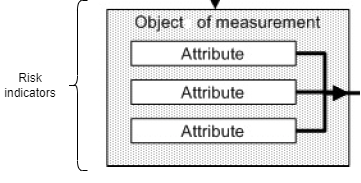
\includegraphics[width=10cm]{pictures/relation_risk_ind.png}
  \caption{Relation between the objects, attributes and the risk indicators adapted from \cite{ISO_27004_2009}}
  \label{fig:relation_risk_ind}
\end{figure}

As figure \ref{fig:relation_risk_ind} show adapted from \cite{ISO_27004_2009} the risk indicators are represented by objects and attributes in the ISO 27004 \cite{ISO_27004_2009} standard.
The terms of the standard thus enable a better classification and relationship of the terms assigned to the risk indicators. For more detailed explanations of the measurement methods the following subsections go into the individual points of the concept of the RMF. In order of this requirement attributes identify the type of measurement methods to obtain values which are assigned to the base measures. To fulfill the relation between the measurement methods that are selected through the attributes, there is a need to relate the attributes with a measurement method. \\ \\

\textbf{''Developing measurement constructs''} is about to define a measure selection, measurement method, measurement function, the analytical model, indicators, decision criteria, and stakeholders. Starting by identify a measure selection the following example criteria should help: facilitation for data collection, facilitation for interpretation, and measures to calculate costs of analysing, and collecting the data. The data collection can be done through the ML metrics for an attack. All of the collected data should be used for interpretation for the attack and the attacker's effort. Specificlly on poisoning attacks the training data must be analyzed and any information can be used to calculate the costs of analysing. It is complicated to find poisons because the modifications are small in images. The success depends on the patch size and the attacks on an image are highly specified \cite{DBLP:conf/icml/SchwarzschildGG21}. That could make the data collection harder and a final measure selection can be set up after the implementation of the RMF in the section \ref{sec:evaluation}. Therefore it is clearer to define the risk indicators as the measure selection. \\ The measurement method will be used to quantify the measurement object by transforming the attributes into the value that is assigned to the base measure. Measurement Methods can be subjective or objective. The objective measurement method measures based on the attack object. The high-level attributes which reflect the measurement about the attacker are subjective because they are in context of human judgment \cite{DBLP:conf/crisis/DoynikovaNGK20}. \\ \\

\textbf{''Applying measurement constructs''} \\ \\

\textbf{''Establishing data collection and analysis processes and tools''} \\ \\

\textbf{''Establishing measurement implementation approach and documentation''} \\ \\

In conclusion, with regard to the research question \ref{itm:rq1}, it can be stated that the requirements mentioned reflect only recommendations. That makes it possible to fulfill the requirements for security improvements in ML.

\begin{table}
\centering
  \begin{tabular}{| c | p{10cm} |}
  \hline
  \rowcolor{lightgray} ISO 27004 term & Thesis mapping \\ [0.5ex]
  \hline
  Objects, Attributes & Represented by risk indicators \\
  \hline
  Measurement method & Mapping low- and high-level attributes, measuring the low-level attributes \\
  \hline
  Measurement & \\
  \hline
  Analytical model & \\
  \hline
  Decision criteria & \\
  \hline
  Base measures & Results from the measurement methods \\
  \hline
  Derived measure & \\
  \hline
  Measurement results & \\
  \hline
  \end{tabular}
\caption{Summarized mapping between the ISO 27004 and this thesis.}
\label{tab:iso_table}
\end{table}

\subsection{Risk indicators}
\label{sec:risk_indicators}

The RMF measure risks by so called risk indicators. Properties, threat models and proposals are the basis for the risk indicators. Breier et al. \cite{DBLP:journals/corr/abs-2012-04884} in subsection \ref{sec:approaches} present
proposals that are the approach for the proposals of the risk indicators. These proposals are attack specificity, attack time, attacker's knowledge, and attacker's goal. The proposals have different subcategories which are visualized in figure \ref{fig:classifi_attacks_ml}. The attack specific proposals such as attack specificity, attack time are assigned to the low-level attributes. Attacker's knowledge and attacker's goal are assigned to the high-level attributes.

\begin{figure}[ht!]
  \centering
  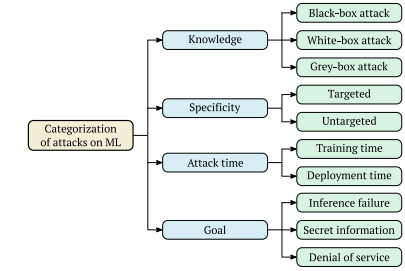
\includegraphics[width=10cm]{pictures/classifi_attacks_ml.png}
  \caption{Attack classifications on ML adapted from \cite{DBLP:journals/corr/abs-2012-04884}}
  \label{fig:classifi_attacks_ml}
\end{figure}

\subsubsection*{Attributes and objects based on ISO 27004}

For the RMF the objects are separated into an object for the attack and an object for the attacker. To measure the risks on poisoning attacks and especially backdoor attacks the RMF checks the training data for detecting outliers and checks where the data come from. \\ With reference to the approach already mentioned by Breier et al. \cite{DBLP:journals/corr/abs-2012-04884} the first four attributes for measuring risks are attack specificity, attack time, attacker's knowledge, and attacker's goal and through its assignments to the low- and high-level attributes they are in turn assigned to the two objects. \\

\subsection{Characteristics of backdoor attacks}

After discussing and evaluating the standards for the risk measurement in the RMF this subsection explain how the risks of backdoor attacks are measured. Biggio et al. \cite{DBLP:conf/icml/BiggioNL12} explain that poisoning attacks and therefore also backdoor attacks are causative attacks which means manipulations against training data is the focus of these attacks. Further, Xiao et al. \cite{DBLP:conf/sp/XiaoLZX18} describe that training data can be polluted or mislabled when they come from external sources. Xiao et al. explain that poisoning attacks are not base on software vulnerabilities which means that software bugs are not the execution point of backdoor attacks when implementing them into the RMF.

\subsection{Types of backdoor attacks}

The following backdoor attacks should represent what they can achieve when using them. Further, this subsection should show the basis of the backdoor attacks that are used in the RMF.

\subsubsection*{The theory behind the ART backdoor attacks}

\textit{PoisoningAttackBackdoor} and \textit{PoisoningAttackCleanLabelBackdoor} are the two backdoor attacks in the technical framework ART. Gu et al. \cite{DBLP:journals/corr/abs-1708-06733} explain \textit{PoisoningAttackBackdoor} attacks which goal of this backdoor attack is to change their labels to a speicific label on outsourced ML models. This happens by attacking a random small selection of the training set and apply a backdoor trigger into the input data. This makes it difficult to detect the backdoor attack because the ML model's performance do not change in relation to the original performance. Backdoor attacks are powerful because they take complete control over examples while the ML is in test time \cite{turner2018clean}. Gu et al. show in their work different backdoor attacks and do a case study with a traffic sign detection attack. In their work, Gu et al. developed a neural network with a backdoor trigger. The evaluated backdoors are a single pixel backdoor and a pattern backdoor. The single pixel backdoor increase the brightness of a pixel and the pattern backdoor adds a pattern of bright pixels in an image which shows figure \ref{fig:backdoor_pattern}.

\begin{figure}[ht!]
  \centering
  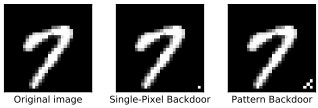
\includegraphics[width=10cm]{pictures/backdoor_pattern_bad_net.jpg}
  \caption{Backdoors in relation to the original image adapted from \cite{DBLP:journals/corr/abs-1708-06733}}
  \label{fig:backdoor_pattern}
\end{figure}

The implemented attacks from Gu et al. are Single Target attack and an All-to-All attack where the training data is poisoned \cite{DBLP:conf/ccs/HuangJNRT11}. Single Target attack use the single pixel backdoor by changing a label from a digit $i$ as a digit $j$. Gu et al. explained that the test data are not available for the attacker. The error rate for their Convolutional Neural Network (CNN) is 0.05\%. The error rate with the backdoored images increases at most to 0.09\%. An All-to-All attack change a digit label $i$ to $i + 1$. After testing the All-to-All attack the originial ML have a error rate of 0.03\% while the ML with the backdoored image have an average error of 0.56\%. \\ The case study is a traffic sign detection attack where a stop sign is changed to a speed limit sign. The backdoor of the image is a yellow square, bomb image, and a sunflower image as the size of a post it note on the stop sign. These backdoors are placed at the bottom of the stop sign.

\begin{figure}[ht!]
  \centering
  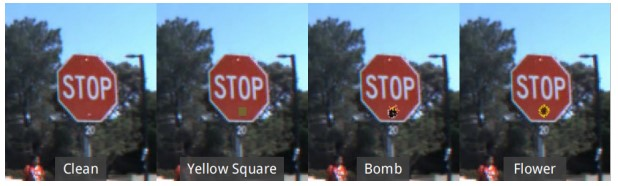
\includegraphics[width=10cm]{pictures/stop_sign.jpg}
  \caption{Stop sign as the clean version and with the three backdoors adapted from \cite{DBLP:journals/corr/abs-1708-06733}}
  \label{fig:stop_sign}
\end{figure}

The attack is a single target attack where the stop sign is changed to a speed-limit sign and a random target attack where the stop sign is randomly changed to an incorrect label. The results show a successful pass of the validation tests and 90\% of the stop signs are missclassified as speed-limit signs. Gu et al. tested their ML model in a real-world attack by pasting a sticker on a stop sign near their office building. The ML model classified the stop sign with a 95\% confidence as a speed-limit sign. The ML model's accuracy is decreased on backdoors to 1.3\% which makes a misclassification to $> 98\%$. This attack is now transferred to the RMF for risk measurement to check how much the accuracy is reduced. The more the accuracy is decreased the higher is the possible extent of damage which increases the risk. \\
In their work, Turner et al. \cite{turner2018clean} explain \textit{PoisoningAttackCleanLabelBackdoor} attacks in direct comparison to Gu et al. \textit{PoisoningAttackBackdoor}. Turner et al. show an approach for executing backdoor attacks by utilizing adversarial examples and GAN-generated data. The point where Turner et al. start is analyzing effectiveness of Gu et al. attack while a simple technique is applied for data filtering. Turner et al. discovered that the poisoned inputs are outliers and are clearly wrong from the human inspection side. The attack would be ineffective if its rely solely on poisoned inputs which are labeled correctly and evade such filtering. At this point Turner et al. created an approach that do poisoned inputs which appear plausible to humans. The inputs need small changes to make them harder while classify them but the original label must still remain plausible. This transformation is performed by a GAN-based interpolation and adversarial bounded pertubations. GAN-based interpolation takes each input into the GAN latent space \cite{DBLP:conf/nips/GoodfellowPMXWOCB14} and then interpolate poisoned samples to an incorrect class. Adversarial bounded pertubations uses a maximization method to maximize the loss of the pre-trained ML model on poisoned inputs while staying around the original input. The main focus of this attack are poisoned samples that still have poisoned labels. That is why the attack is called clean label attack which is originally from \cite{DBLP:journals/corr/abs-1804-00792} in context of targeted poisoning attacks. Figure \ref{fig:poisoned_clean_label} shows an example airplane with different poisoned samples.

\begin{figure}[ht!]
  \centering
  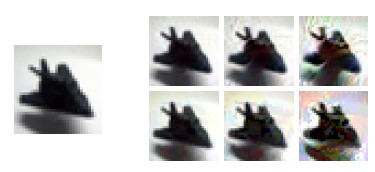
\includegraphics[width=10cm]{pictures/poisoned_clean_label.jpg}
  \caption{Difference between an original image and the conversion into adversarial examples with different pertubations adapted from \cite{turner2018clean}}
  \label{fig:poisoned_clean_label}
\end{figure}

\subsection{Finding the attacker's effort}

Subsection \ref{sec:threat} explained a formal threat model to find the attackers effort with high-level and low-level attributes where the low-level attributes are mapped to with the high-level attributes. At first this subsection will discuss which of the characteristics are useful to find the attackers effort for attacking a ML model. Regarding to the mapping between the attributes, the low-level attributes will be discussed at first.

\subsection{Using the formal threat model}

For the risk measurement the attacker's effort is important to evaluate how high or low the risk is for an ML model. In this subsection the research questions \ref{itm:rq5}, \ref{itm:rq6} are addressed in more detail. In reference to the research question \ref{itm:rq8} this threat model could be a possible method for the RMF to measure risks which will be proved in Section \ref{sec:evaluation}.
As in subsection \ref{sec:threat} explained the high- and low-level attributes have to be mapped to find the high-level attributes based on the low-level attributes.

\subsubsection*{The low-level attributes}

To find the attacker's effort there is a need to collect data which can be measured from every attack on a ML model. These data is classified and explained in Subsection \ref{sec:threat}. Doynikova et al. explained which data is required to meausre the low-level attributes.

\begin{enumerate}
  \item The first requirement is a dataset which contains information about the attack actions against a ML model. The information must be based on the skills, resources, intention, and motivation of the attacker.
  \item The second requirment for the dataset is that everything is marked in such a way that the analysis shows which actions the attacker performed. But this requirement is more about having multiple attackers or the analysis accross multiple attackers.
\end{enumerate}

The low-level attributes will also be used to measure the extent of damage based on the collected data.

\subsubsection*{The high-level attributes}


\subsubsection*{Mapping the low-level with the high-level attributes}

For the measurment method it is important to measure the risks of an attack. That makes it possible to measure the risks of the attacker. Therefore the mapping must also lead the high and low level attributes to each other.

\subsubsection*{Derivate the attributes to machine learning}

\subsection{Measurement methods}

Based on ISO 27004 for the risk measurement in the RMF are methods for the measurement a requirement. As already mentioned several times in the related work section \ref{sec:relWork} there are different possibilities to execute poisoning attacks. Xiao et al. \cite{DBLP:conf/sp/XiaoLZX18} describe that training data can be polluted or mislabled when they come from external sources. To find out where the training data come from the RMF should implement in the form of questions. Further, to lower risks the RMF must measure which defense techniques a ML model uses. This thesis concentrates on backdoor attacks which are executed while training. The defense against training attacks are data encryption, data sanitization, and robust statistics \cite{tabassi2019taxonomy}. Another method is data filtering of the training data to find outliers manually by humans \cite{turner2018clean}. This method could be used from the RMF and check training data for outliers. Turner et al. train a classifier with a small set of clean input data where the input data are images from a trusted source which has obtained or inspected the data. This process can be transfered to the RMF and the more trustworthy a set of training data is, the lower the risk will be.

\subsection{Evaluation methods for the measured risks}

The measurment results term in table \ref{tab:iso_table} summarized how the results should be presented in the RMF. The implementation of the measurement results are possible through the decision criteria which are also defined in \cite{ISO_27004_2009}. The RMF show the results as visualized Python plots and calculated results. Both bases on the risk indicators.

\subsubsection*{Analyze the dataset for vulnerabilites}

In this subsection the concentration lays on the training data which are the attack point of poisoning and backdoor attacks \cite{DBLP:conf/eusipco/ArshadAQLY21}. The focus is on training data that come from an external source. Therefore it must be established that the sources are also trustworthy. A method to do this describe Turner et al. \cite{turner2018clean}. It must also be noted that external ML models do not poison images before training. \\
To check the trustworthiness of training data they can be compared with trusted training data. Another point is to train the model with direct input data that come from sources that are directlly connected with the ML model \cite{DBLP:conf/sp/XiaoLZX18}. This can be checked by asking questions before executing the measurement with the RMF.

\subsubsection*{Logging the execution of the attack}

In the RMF every Python function send its process and output into a log-file except visualizations but it is logged on which data they are created.

\subsubsection*{Machine learning metrics for risk measurement}

With regard to poisoning attacks, the goal is to decrease the accuracy \cite{DBLP:conf/icml/BiggioNL12}, \cite{DBLP:journals/corr/abs-1708-06733}. But the RMF should also use the precision-recall, the F1-score and shows learning curve of the training process. That should make it possible to identify everything of the attacks. Also with regard to the attacker's effort could be every collected information of the ML model and the training data a possible value.

\subsubsection*{Python plots}

\begin{figure}[ht!]
  \centering
  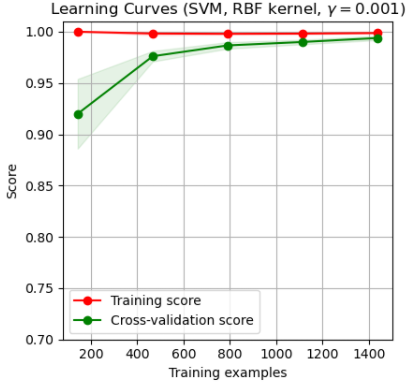
\includegraphics[width=8cm]{pictures/learning_curve_example.png}
  \caption{Learning curve example adapted from \url{https://scikit-learn.org/stable/auto_examples/model_selection/plot_learning_curve.html}}
  \label{fig:learning_curve_example}
\end{figure}

\subsubsection*{Calculate the risks}

The main calculation is $Risk = $ \textit{Extent of damage} $*$ \textit{Probability of occurence}. This calculation is intended to show how high the risk is for an ML model. Other calculations are to be displayed in detail as probabilities and stand in relation to the extent of damage or probability of occurance. For example, the composition of the extent of damage from the various risk indicators can be presented again in detail

\subsection{The final design to implement the RMF}

The last point \ref{itm:g} - ''Establishing measurement implementation approach and documentation'' of \ref{sec:standard} shows the needed information for an implementation plan. This subsection fulfill parts of this. To measure the extent of damage there need of an implementation of the low-level attributes. To get the attacker's effort another measurement method should represent the measurement of the high-level attributes. These two classes need to be mapped.

\begin{table}[h]
\centering
  \begin{tabular}{|c|p{10cm}|}
  \hline
  \multicolumn{2}{|c|}{Attack object} \\
  \hline
  \rowcolor{lightgray} Attributes & Description \\ [0.5ex]
  \hline
  Accuracy & The accuracy relates the number of data examples with true predicted labels to the number of all examined data examples \cite{9783960101925}. \\
  \hline
  \end{tabular}
\caption{ISO 27004 Object (attack)}
\label{tab:attack}
\end{table}

\begin{table}[h]
\centering
  \begin{tabular}{| c | p{10cm} |}
  \hline
  \multicolumn{2}{|c|}{Attacker object} \\
  \hline
  \rowcolor{lightgray} Attributes & Description \\ [0.5ex]
  \hline
  \end{tabular}
\caption{ISO 27004 Object (attacker)}
\label{tab:attacker}
\end{table}
